\section{System Architecture}
The system is designed with a strict modular approach, ensuring individual components can evolve independently. The Database Layer utilizes PostgreSQL as the central reliable storage mechanism. Ingestion processes handle both historical data seeds and automated pipelines that extract unstructured transactions from emails and PDFs.

Figure \ref{fig:arch} illustrates the holistic Data Flow. Extracted data undergoes a robust ETL layer to patch structural and historical inconsistencies. The Feature Store systematically transforms transactional records into continuous Time-series Panels. All forecasting artifacts are eventually exported as CSV datasets and accessible SQL Views.

\begin{figure}[H]
\centering
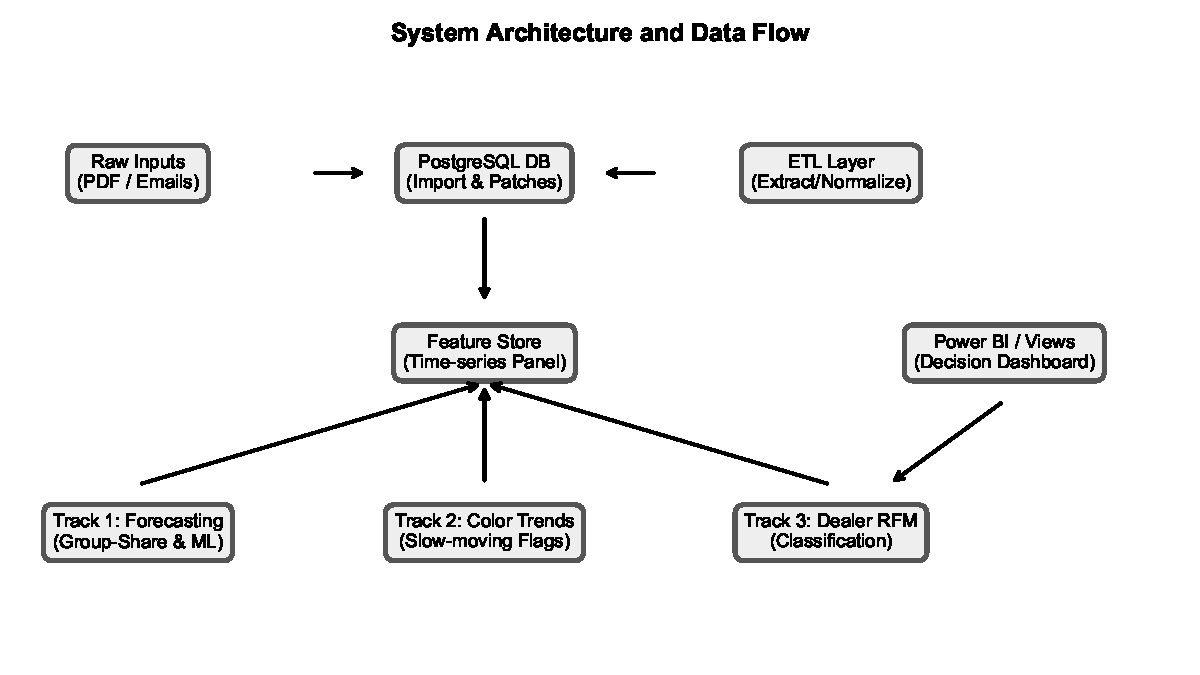
\includegraphics[width=0.85\textwidth]{../figures/en/architecture.pdf}
\caption{System Architecture and Data Flow Diagram}
\label{fig:arch}
\end{figure}

The clear separation of concerns inherent in this layered architecture supports maintainability and codebase reusability for future cyclical updates.
\FloatBarrier
